\documentclass[11pt,a4paper]{article}
\usepackage[spanish]{babel}
\usepackage[utf8]{inputenc}
\usepackage[margin=2cm]{geometry}
\usepackage{graphicx}
\usepackage{float}
\title{\textbf{Anexo --- La \'ultima transmisi\'on}\\ \large Diagramas y evidencia del tablero}
\author{Daniel Sanchez --- Juan Diego Serpa}
\date{\today}
\newcommand{\figura}[3]{\begin{figure}[H]\centering\includegraphics[width=#2\linewidth,height=0.38\textheight,keepaspectratio]{#1}\caption{#3}\end{figure}}
\newcommand{\captura}[2]{\IfFileExists{#1}{\begin{figure}[H]\centering\includegraphics[width=0.95\linewidth,height=0.4\textheight,keepaspectratio]{#1}\caption{#2}\end{figure}}{\fbox{\parbox{0.9\linewidth}{\textbf{PENDIENTE:} colocar aqu\'i la captura \texttt{#1}.}}}}
\begin{document}
\maketitle
\section*{A. Modelos (U5)}
\figura{GRAFICOS/CONTEXTO.png}{0.8}{Diagrama de contexto}
\figura{GRAFICOS/CASOS DE USO.png}{0.8}{Casos de uso}
\figura{GRAFICOS/CLASES.png}{0.8}{Clases del dominio}
\figura{GRAFICOS/SECUENCIA.png}{0.9}{Secuencia de elegir una opci\'on}
\figura{GRAFICOS/ESTADOS.png}{0.95}{Estados de una sesi\'on}
\section*{B. Arquitectura (U6)}
\begin{figure}[H]\centering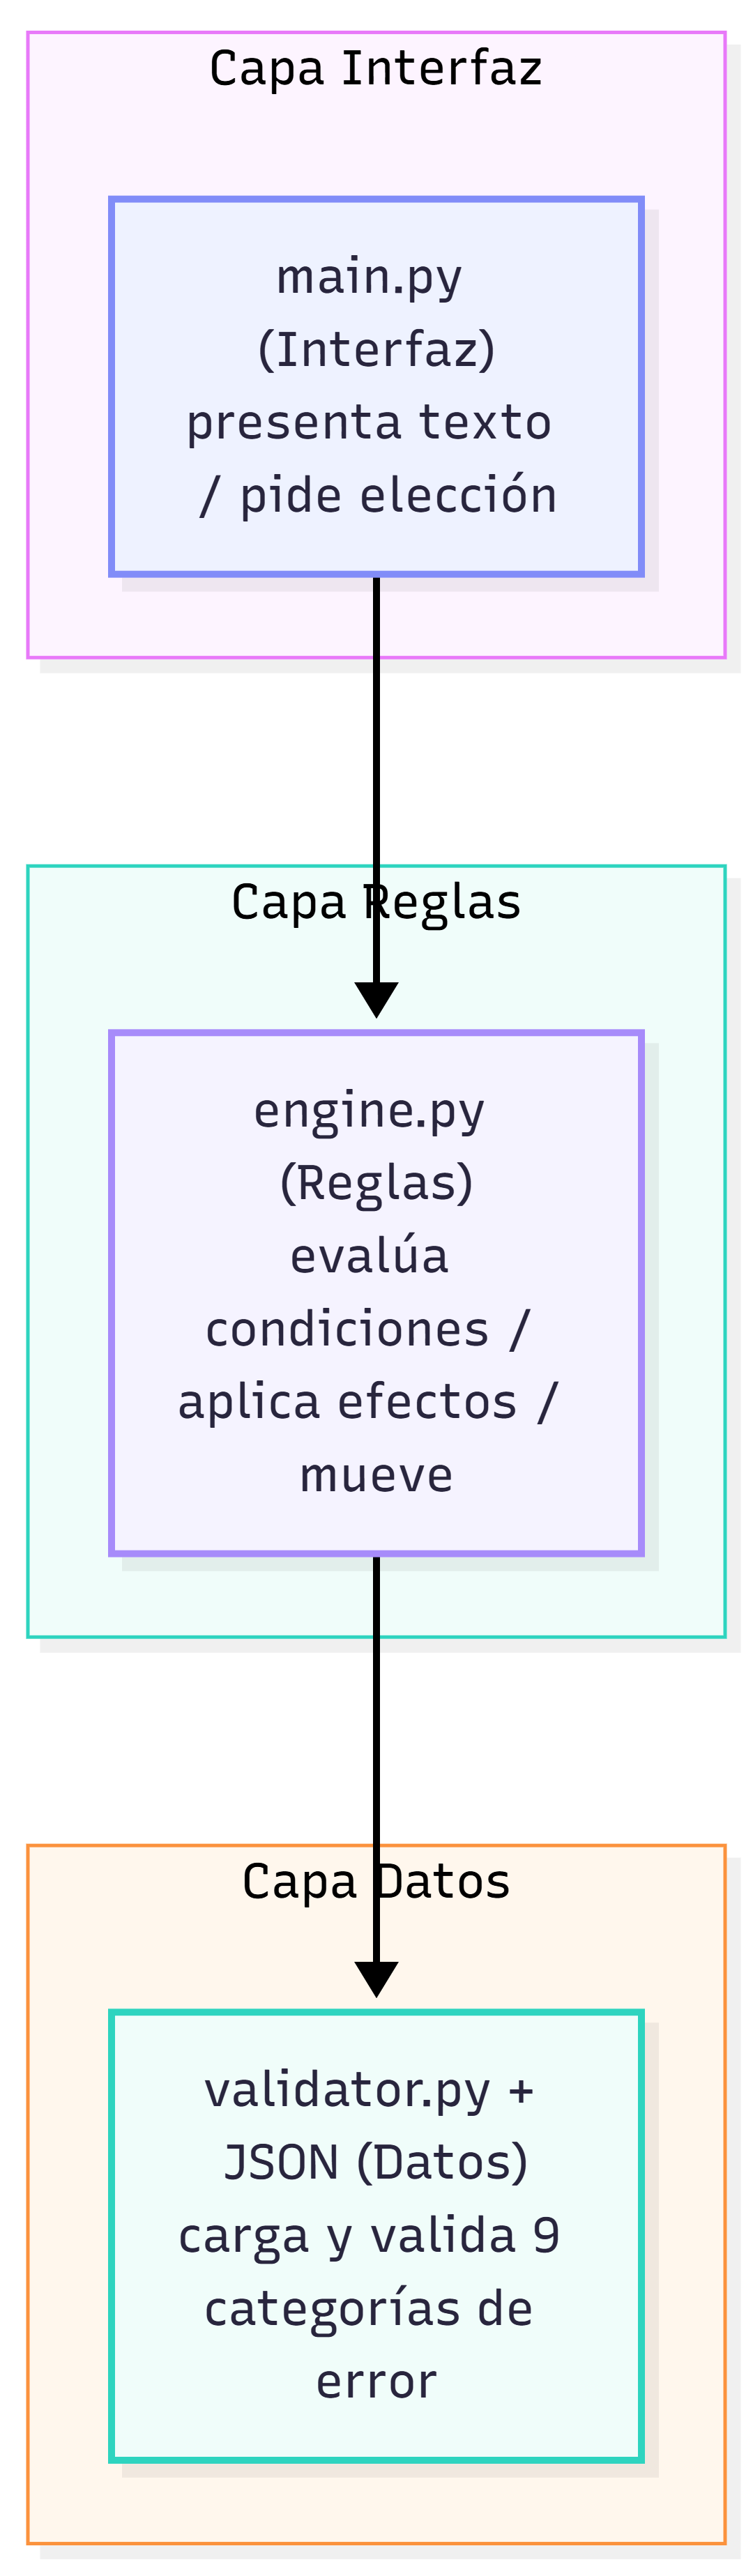
\includegraphics[height=0.5\textheight,keepaspectratio]{GRAFICOS/COMPONENTES.png}\caption{Componentes: Interfaz (\texttt{main.py}) $\to$ Reglas (\texttt{engine.py}) $\to$ Contenido (\texttt{validator.py} + JSON)}\end{figure}
\section*{C. Tablero Kanban (U3)}
\captura{tablero_inicial.png}{Tablero al inicio del trabajo}
\captura{tablero_final.png}{Tablero al cierre}
\end{document}
